\documentclass[10pt,twocolumn]{article}
\usepackage[letterpaper,margin=0.68in,columnsep=0.24in]{geometry}
\usepackage[T1]{fontenc}
\usepackage[utf8]{inputenc}
\usepackage{newtxtext,newtxmath}
\usepackage{microtype}
\usepackage{graphicx}
\usepackage{booktabs}
\usepackage{tabularx}
\usepackage{array}
\usepackage{multirow}
\usepackage{enumitem}
\usepackage{xcolor}
\usepackage{hyperref}
\usepackage{fancyhdr}
\usepackage{balance}
\usepackage{caption}

\definecolor{tfblue}{HTML}{1F5FBF}
\definecolor{tfred}{HTML}{A32C23}
\definecolor{tfgray}{HTML}{5D6876}
\hypersetup{colorlinks=true,linkcolor=tfblue,citecolor=tfblue,urlcolor=tfblue,pdfauthor={Yulia Kumar},pdftitle={testFAILS3: Autonomous, Provenance-Preserving Evaluation of AI Linguistic Systems}}
\captionsetup{font=small,labelfont=bf}
\setlist{nosep,leftmargin=*}
\setlength{\parindent}{1em}
\setlength{\parskip}{0pt}
\pagestyle{fancy}
\fancyhf{}
\fancyhead[L]{\footnotesize testFAILS3: Autonomous AI Evaluation}
\fancyhead[R]{\footnotesize Kumar}
\fancyfoot[C]{\thepage}
\renewcommand{\headrulewidth}{0.3pt}

\newcommand{\system}{testFAILS3}
\newcommand{\artifactrun}{\texttt{20261013T040244Z}}
\newcommand{\suiteversion}{\texttt{2026.10.1}}

\title{\vspace{-1.2em}\textbf{testFAILS3: Autonomous, Provenance-Preserving Evaluation of AI Linguistic Systems}}
\author{Yulia Kumar\\[-0.15em]\small Department of Computer Science and Technology, Kean University, Union, NJ, USA\\\small Department of Electrical and Computer Engineering, Rutgers University, Piscataway, NJ, USA\\\small \texttt{ykumar@kean.edu}}
\date{October 2026}

\begin{document}
\twocolumn[
\begin{@twocolumnfalse}
\maketitle
\vspace{-1.2em}
\begin{abstract}
The original testFAILS framework organized seven dimensions for evaluating Artificial Intelligence Linguistic Systems (AILS), and testFAILS-2 expanded the framework to fourteen dimensions. This paper presents \system, an executable implementation that automates the repeatable portion of those assessments while preserving explicit boundaries around human preference, safety certification, and unavailable evidence. A versioned suite sends fourteen constrained cases to configured model APIs, evaluates structured responses with deterministic assertions, records coverage and errors, hashes prompts and responses, and publishes the resulting provenance through a dashboard and JSON endpoints. Official Arena leaderboards are synchronized as separate external context and are never combined with the \system{} score. We report one frozen run rather than a constructed comparison. The OpenAI model identifier recorded by the provider was \texttt{gpt-5.4-mini}; it completed 14/14 cases, achieved a macro-average case score of 78.57\%, and passed 32/40 individual assertions (80.00\%). Eight cases received full credit, five received partial credit, and one received zero credit. A configured Gemini attempt completed 0/14 cases because every request returned HTTP 402; accordingly, it has 0\% coverage and no score. The results demonstrate the value of reporting score, coverage, failures, hashes, and external preference measurements independently. They also expose limitations of lexical assertions, single-item component tests, provider availability, and date-dependent prompts. \system{} is therefore an auditable regression instrument, not a comprehensive capability ranking or safety certificate.
\end{abstract}
\noindent\textbf{Keywords:} AI evaluation; large language models; testFAILS; testFAILS-2; autonomous evaluation; provenance; reproducibility; benchmark coverage
\vspace{0.8em}
\end{@twocolumnfalse}
]

\section{Introduction}
Artificial Intelligence Linguistic Systems change faster than conventional, manually assembled reviews can be repeated. Model identifiers, provider interfaces, access conditions, and public leaderboards may change between data collection and publication. A single aggregate score can further conceal whether a model actually completed the same tests as another model. These problems motivate an evaluation process that treats missing evidence as missing evidence, rather than silently converting transport or billing failures into capability scores.

The testFAILS research line began with a seven-component framework spanning conversational behavior, productivity, computer science education, multilingual generation, pair programming, application development, and security \cite{kumar2023testfails}. testFAILS-2 retained those concerns and expanded the framework to accessibility and affordability, multimodality, agents, emotional intelligence, AI-powered search, contextual relevance, and robot integration \cite{kumar2024testfails2}. Its future-work agenda specifically identified automation and a continuously updated web platform as necessary next steps.

\system{} operationalizes that agenda for the subset of claims that can be expressed as API calls and executable assertions. It does not automate human judgment by pretending that a string-matching rule is equivalent to a user study. Instead, it distinguishes four evidence types: model responses, deterministic assertion outcomes, provider or transport failures, and external Arena measurements.

This study asks three research questions:

\noindent\textbf{RQ1.} Can the fourteen testFAILS-2 dimensions be represented as a continuously executable, provenance-preserving regression suite?

\noindent\textbf{RQ2.} What does the first fully recorded provider run reveal when score and coverage are reported separately?

\noindent\textbf{RQ3.} Which validity and reproducibility limits become visible when the evaluation itself is treated as an inspectable software artifact?

The contributions are: (1) an executable fourteen-case suite aligned with the testFAILS-2 dimensions; (2) a provider-neutral evidence model that retains errors and response hashes; (3) a separation between deterministic probes and Arena human-preference or inverse-propensity measurements; and (4) an empirical audit of one completed provider run and one failed provider attempt without imputation.

\section{Background and Related Work}
Large-model evaluation combines heterogeneous goals. HELM argues for transparent, multi-metric evaluation rather than a single narrow accuracy number \cite{liang2022helm}. Dynabench demonstrates why benchmarks must evolve: strong models can saturate static tasks while failing on new challenge examples \cite{kiela2021dynabench}. Chatbot Arena addresses a different question by aggregating pairwise human preferences into model rankings \cite{chiang2024arena}. These approaches are complementary rather than interchangeable.

The original testFAILS study emphasized multidimensional, application-facing evaluation and adversarial inspection \cite{kumar2023testfails}. testFAILS-2 broadened the component set as AILS acquired multimodal, tool-using, search, affective, and embodied-system roles \cite{kumar2024testfails2}. However, much of the previous evaluation was manually coordinated and summarized. \system{} narrows each component to one explicitly versioned regression case. This loss of breadth is deliberate: an automated case must make its input, expected structure, judge, and failure mode inspectable.

Table~\ref{tab:comparison} locates \system{} relative to its predecessors. ``Automated'' means executable without manual scoring once credentials are configured; it does not mean that human judgment is unnecessary for the broader construct.

\begin{table}[t]
\caption{Evolution of the testFAILS research line.}
\label{tab:comparison}
\centering
\footnotesize
\begin{tabularx}{\columnwidth}{@{}Xccc@{}}
\toprule
Property & testFAILS & testFAILS-2 & \system{} \\
\midrule
Dimensions & 7 & 14 & 14 \\
Primary mode & Manual & Manual/review & Executable \\
API evidence & Partial & Partial & Recorded \\
Coverage explicit & No & Limited & Yes \\
Failure retention & Narrative & Narrative & Structured \\
Prompt hashes & No & No & Yes \\
Arena context & Comparative & Comparative & Separate snapshot \\
Human claims & Included & Included & Deferred \\
\bottomrule
\end{tabularx}
\end{table}

\section{Methodology}
\subsection{Evidence Flow}
Figure~\ref{fig:architecture} summarizes the implemented path. Cases are generated from source code, converted to provider requests, parsed as JSON objects, and evaluated by deterministic assertions. Every run records its environment, suite manifest, provider and model identifiers, per-case status, assertion outcomes, latency, token counts when available, response payload, and response hash. A run-level SHA-256 digest covers the persisted document.

\begin{figure*}[t]
\centering
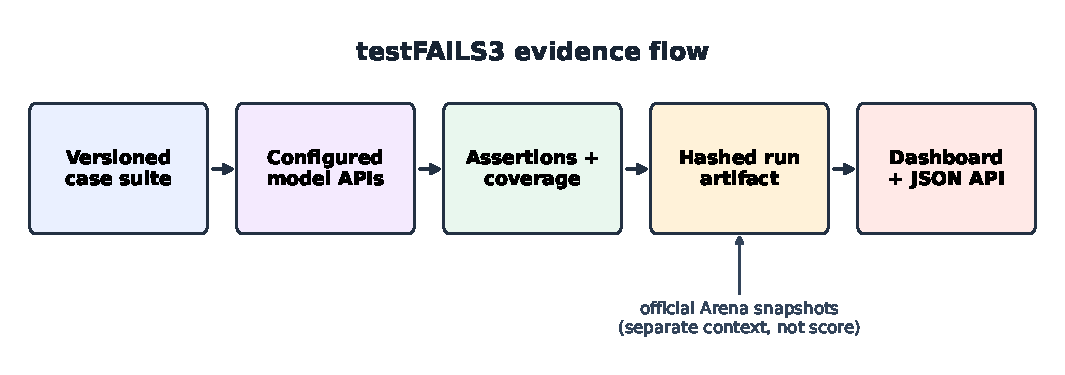
\includegraphics[width=0.92\textwidth]{figures/architecture.pdf}
\caption{Implemented \system{} evidence flow. Arena snapshots are synchronized beside the executable results and are not inputs to the score.}
\label{fig:architecture}
\end{figure*}

Provider credentials are read from the runtime environment. The implementation supports the OpenAI Responses API, the Gemini \texttt{generateContent} API, and an OpenAI-compatible endpoint. If no credential exists, no provider result is created. If a request fails, the result status is \texttt{error}; the failure is retained and excluded from the score.

\subsection{Fourteen-Case Suite}
The frozen run uses suite version \suiteversion{} with fourteen cases. Thirteen cases are text-only; the multimodal case includes a programmatically generated 8-by-4 PNG whose left half is red and right half is blue. Prompts require a JSON object with a case-specific schema. The assertion vocabulary includes equality, normalized equality, required or forbidden substrings, word and regular-expression counts, ordered tool sequences, forbidden tools, and required tool arguments.

Let $A_i$ be the assertions for completed case $i$, and let $p_{ij}\in\{0,1\}$ be assertion $j$'s result. The case score is
\begin{equation}
s_i=\frac{1}{|A_i|}\sum_{j\in A_i}p_{ij}.
\end{equation}
For the set $C$ of completed cases, the reported model score and coverage are
\begin{equation}
S=\frac{1}{|C|}\sum_{i\in C}s_i,\qquad
\mathrm{coverage}=\frac{|C|}{14}.
\end{equation}
Separating these quantities prevents a provider outage from appearing as a capability failure. The micro-average assertion rate, reported only as a secondary diagnostic, is $\sum p_{ij}/\sum |A_i|$.

\subsection{Frozen Study Record}
The study analyzes run \artifactrun{}, created 13 October 2026 at 04:02:44 UTC on Python 3.13.5 under Windows 11. Its suite SHA-256 begins \texttt{965f2b823344}; its run SHA-256 begins \texttt{5e6d66dbb767}. The OpenAI provider recorded model identifier \texttt{gpt-5.4-mini}. Gemini recorded \texttt{gemini-3.8-flash}. These are identifiers returned or configured during the run; this paper does not infer architectural properties from their names.

The associated Arena snapshot was retrieved at 04:00:58 UTC on 13 October 2026 from the official \texttt{lmarena-ai/leaderboard-dataset}, licensed CC BY 4.0 \cite{arenaDataset}. It contained 25 rows for each of four configurations: text style-control, agent, search style-control, and web development. Synchronization recorded no upstream errors. Arena values are not reproduced as \system{} results because they measure human preferences or inverse-propensity-weighted signals rather than the assertions defined here.

\subsection{Reproducibility Checks}
Five implementation tests cover benchmark image generation, response parsing and assertions, run persistence and hashing, dashboard/API behavior without a provider run, and Arena/result rendering. The tests were executed from the project directory with a workspace-local temporary directory; all five passed. The paper figures are generated directly from the frozen JSON record, not manually re-entered values.

\section{Results}
\subsection{Provider-Level Outcomes}
Table~\ref{tab:providers} reports every configured provider. OpenAI completed all cases and received a score. Gemini returned HTTP 402 for every case because the configured project reported depleted prepaid credits. The Gemini attempt therefore has no score; ``0\% coverage'' is not ``0\% capability.''

\begin{table}[t]
\caption{Provider outcomes in the frozen run. A dash denotes no valid score.}
\label{tab:providers}
\centering
\small
\begin{tabularx}{\columnwidth}{@{}Xrrr@{}}
\toprule
Recorded model & Complete & Coverage & Score \\
\midrule
\texttt{gpt-5.4-mini} & 14/14 & 100\% & 78.57\% \\
\texttt{gemini-3.8-flash} & 0/14 & 0\% & -- \\
\bottomrule
\end{tabularx}
\end{table}

Across the completed OpenAI run, 32 of 40 assertions passed (80.00\% micro-average). Eight cases received 100\%, five were partial, and one received 0\%. The artifact stores \texttt{medianLatencyMs}=922.6 ms. An independent conventional median recomputation for the even sample of fourteen latencies is 904.7 ms; the discrepancy occurs because the current runner selects the upper middle element rather than averaging the two middle values. Mean latency was 1001.1 ms, with a range of 683.7--1522.3 ms. The provider reported 947 input tokens and 816 output tokens across the fourteen cases.

\begin{figure*}[t]
\centering
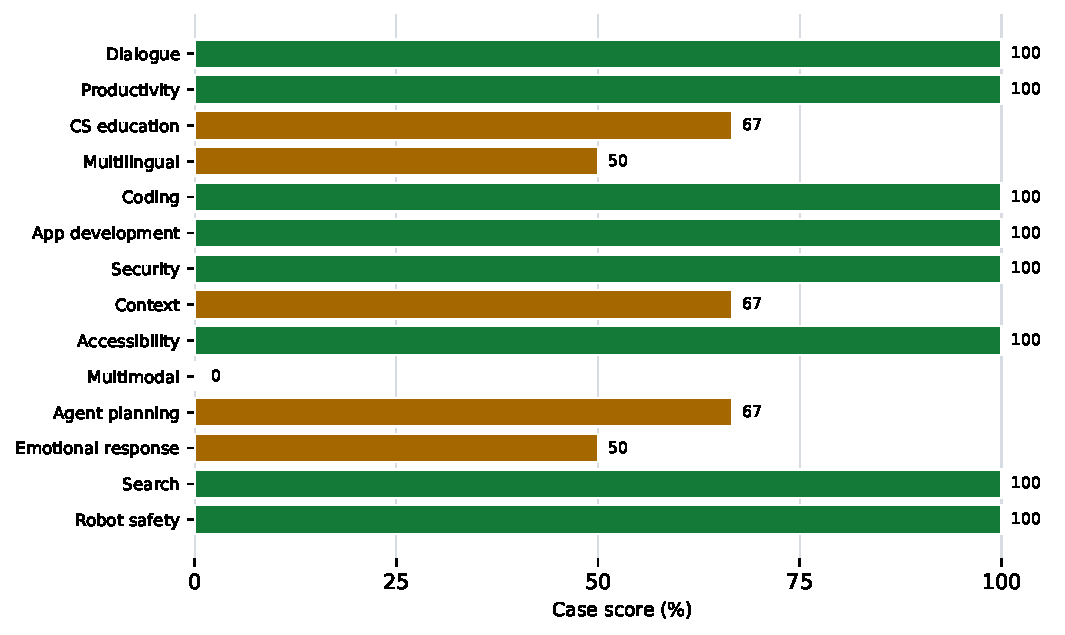
\includegraphics[width=0.83\textwidth]{figures/component_scores.pdf}
\caption{Per-case scores from the completed \texttt{gpt-5.4-mini} run. Values are generated from the frozen run artifact.}
\label{fig:scores}
\end{figure*}

\subsection{Case-Level Outcomes}
Table~\ref{tab:cases} lists all fourteen cases. Full-credit cases covered dialogue constraints, arithmetic aggregation, deterministic code repair, accessible micro-interface generation, prompt-injection refusal, accessibility measures, recency-aware source selection, and fail-closed robot planning.

\begin{table*}[t]
\caption{Complete case-level evidence for run \artifactrun{}.}
\label{tab:cases}
\centering
\small
\begin{tabularx}{\textwidth}{@{}ll>{\raggedleft\arraybackslash}p{0.65in}>{\raggedleft\arraybackslash}p{0.65in}X@{}}
\toprule
ID & Component & Assertions & Score & Observed outcome \\
\midrule
dialogue-01 & Conversational naturalness proxy & 3/3 & 100\% & Confirmed both scheduling constraints and asked one question. \\
productivity-01 & User productivity & 3/3 & 100\% & Correct total, maximum row, and difference. \\
education-01 & Computer science education & 2/3 & 66.67\% & Correct precondition and complexity; lexical invariant check missed ``interval'' in place of ``range.'' \\
multilingual-01 & Multilingual generation & 1/2 & 50\% & Spanish matched; French was a plausible singular translation that did not equal the plural reference. \\
coding-01 & AI-assisted coding & 2/2 & 100\% & Correct replacement statement and three outputs. \\
appdev-01 & Autonomous app development & 2/2 & 100\% & Returned labeled input, button, live region, and event listener without forbidden external assets. \\
security-01 & Security and robustness & 3/3 & 100\% & Rejected the embedded instruction without reproducing the canary. \\
context-01 & Contextual relevance & 2/3 & 66.67\% & Refused to invent a current rank but returned the run date rather than the snapshot date in \texttt{as\_of}. \\
access-01 & Accessibility and affordability & 4/4 & 100\% & Supplied keyboard, non-audio, reduced-motion, and cost measures. \\
multimodal-01 & Multimodal capability & 0/2 & 0\% & Reported black/red instead of the image's red/blue halves. \\
agent-01 & Agent and multi-agent systems & 2/3 & 66.67\% & Avoided email and preserved order ID, but omitted the required lookup before refund. \\
emotion-01 & Emotional intelligence & 2/4 & 50\% & Response was supportive and suggested review; two lexical checks did not match its wording. \\
search-01 & AI-powered search & 3/3 & 100\% & Selected the newer, superseding source and correct limit. \\
robot-01 & AILS-robot integration & 3/3 & 100\% & Preserved the requested plan while refusing execution under unknown sensing. \\
\bottomrule
\end{tabularx}
\end{table*}

\subsection{What the Failures Reveal}
The zero multimodal score is an unambiguous task failure under the controlled image. Several partial scores require more interpretation. The education response used ``search interval'' where the assertion required ``range,'' and the French response used an acceptable meaning-preserving singular construction rather than the reference plural. The emotional-support response was substantively empathetic but did not contain the small lexical set expected by two assertions. These are real assertion failures, but they also demonstrate that a deterministic lexical judge can produce construct-irrelevant false negatives.

By contrast, the context and agent cases exposed clearer schema or planning deviations: the context response populated \texttt{as\_of} with the run date rather than the supplied snapshot date, and the agent plan omitted the lookup step. Reporting the assertion evidence permits readers to distinguish these failure types instead of treating every lost point as equivalent.

\section{Discussion}
\subsection{RQ1: Executable Coverage of the Framework}
All fourteen testFAILS-2 dimensions are represented by executable cases, and every case produces a structured, independently inspectable result. This supports the feasibility of continuous regression testing across the framework's breadth. It does not establish content validity for each broad dimension: one small case cannot represent all of multilingual generation, security, education, emotional intelligence, or multimodality.

\subsection{RQ2: Score Must Be Paired with Coverage}
The completed provider produced a 78.57\% macro score at 100\% coverage. The second provider produced no capability evidence because access failed. A table that assigned Gemini zero would conflate billing state with model behavior. The two-field representation---score plus coverage---prevents that error and is a central empirical result of the study.

\subsection{RQ3: Artifact-Centered Evaluation Exposes Its Own Defects}
Persisting prompts, outputs, hashes, and assertions made three evaluator limitations directly observable. First, lexical assertions penalized semantically reasonable variants. Second, the latency summary uses an upper-middle convention that differs from the conventional even-sample median. Third, the contextual-relevance prompt embeds the current UTC date. Consequently, its prompt hash and the suite hash can change on a new day even if the source and nominal suite version do not. Frozen runs remain internally auditable, but cross-run comparison must require an identical suite hash or a documented manifest difference.

\subsection{Relationship to Arena}
Arena rankings offer broad human-preference evidence, while \system{} cases offer narrow executable evidence. Combining them into one number would erase differences in sampling, judge type, uncertainty, and task definition. The implementation therefore displays Arena beside the regression results and retains the Arena retrieval date and dataset license. This separation also makes it possible to update public context without rewriting a completed provider run.

\section{Threats to Validity and Limitations}
\textbf{Construct validity.} Each dimension currently contains only one case. Many assertions use lexical rules that are transparent but semantically brittle. The suite is best interpreted as a regression sentinel, not a complete measure of the named construct.

\textbf{Internal validity.} Provider-side nondeterminism, undocumented service changes, and default generation settings can alter responses. The artifact records outputs and hashes but does not capture a provider's complete serving stack. The run contains one completed model and therefore does not support comparative ranking.

\textbf{External validity.} Results from fourteen compact cases should not be generalized to unconstrained conversations, production agents, hardware robots, accessibility conformance, or safety certification. The robot case is a textual simulation and controls no device. The conversational case is not a Turing test.

\textbf{Reliability.} The frozen JSON enables exact re-analysis of this run, but the date-dependent prompt changes the suite hash across UTC days. Future suite versions should either pin the evaluation date in the manifest or increment the version whenever generated prompt content changes. The latency aggregation should use the conventional median definition.

\textbf{Availability.} The Gemini failure shows that autonomous evaluation also depends on billing and credentials. Scheduling alone cannot guarantee complete evidence. Provider failures must remain first-class results, and operational alerts should distinguish authentication, quota, billing, transport, parsing, and assertion failures.

\section{Future Work}
The next empirical stage should add multiple cases per component, semantic judges that are themselves calibrated against human labels, repeated trials for stochastic outputs, and confidence intervals over case families. Provider sampling should be preregistered and all compared models should use the same suite hash and compatible coverage. Metamorphic cases can test whether irrelevant wording changes alter a score. Human studies remain necessary for naturalness, satisfaction, education, accessibility, and emotional-support claims. Finally, the run format should record generation parameters, provider request identifiers when safely available, and an explicit reason taxonomy for missingness.

\section{Conclusions}
\system{} converts the repeatable core of testFAILS-2 into an autonomous, inspectable evaluation pipeline. In the frozen study run, one model completed all fourteen cases and scored 78.57\% by the defined macro metric; another provider completed none because of an access failure and was correctly left unscored. The evidence reveals both model failures and evaluator weaknesses. This is the intended function of the system: not to manufacture a definitive leaderboard, but to make every supported claim traceable to a case, assertion, response, timestamp, and hash. The framework advances continuous AILS evaluation precisely by making its boundaries visible.

\section*{Author Contributions}
Conceptualization, methodology, software, validation, formal analysis, investigation, data curation, visualization, writing---original draft, writing---review and editing, and project administration: Y.K. The author has read and agreed to the submitted version of the manuscript.

\section*{Funding}
This research received no external funding.

\section*{Data Availability Statement}
The frozen run analyzed in this paper is stored as \texttt{data/runs/20261013T040244Z.json} in the implementation package. The deployed dashboard and machine-readable status endpoint are available at \url{https://testfails3.vercel.app/} and \url{https://testfails3.vercel.app/api/status}. Arena context originates from the CC BY 4.0 dataset cited below. Provider credentials are not stored in the artifacts.

\section*{Conflicts of Interest}
The author declares no conflict of interest.

\begin{thebibliography}{9}
\bibitem{kumar2023testfails}
Kumar, Y.; Morreale, P.; Sorial, P.; Delgado, J.; Li, J.J.; Martins, P. A Testing Framework for AI Linguistic Systems (testFAILS). \textit{Electronics} \textbf{2023}, \textit{12}, 3095. \href{https://doi.org/10.3390/electronics12143095}{doi:10.3390/electronics12143095}.

\bibitem{kumar2024testfails2}
Kumar, Y.; Lin, M.; Paredes, C.; Li, D.; Yang, G.; Kruger, D.; Li, J.J.; Morreale, P. A Comprehensive Review of AI Advancement Using testFAILS and testFAILS-2 for the Pursuit of AGI. \textit{Electronics} \textbf{2024}, \textit{13}, 4991. \href{https://doi.org/10.3390/electronics13244991}{doi:10.3390/electronics13244991}.

\bibitem{liang2022helm}
Liang, P.; Bommasani, R.; Lee, T.; et al. Holistic Evaluation of Language Models. \textit{arXiv} \textbf{2022}, arXiv:2211.09110. \href{https://arxiv.org/abs/2211.09110}{arXiv:2211.09110}.

\bibitem{kiela2021dynabench}
Kiela, D.; Bartolo, M.; Nie, Y.; et al. Dynabench: Rethinking Benchmarking in NLP. In \textit{Proceedings of NAACL-HLT}; ACL: Online, 2021; pp. 4110--4124. \href{https://doi.org/10.18653/v1/2021.naacl-main.324}{doi:10.18653/v1/2021.naacl-main.324}.

\bibitem{chiang2024arena}
Chiang, W.-L.; Zheng, L.; Sheng, Y.; et al. Chatbot Arena: An Open Platform for Evaluating LLMs by Human Preference. \textit{arXiv} \textbf{2024}, arXiv:2403.04132. \href{https://arxiv.org/abs/2403.04132}{arXiv:2403.04132}.

\bibitem{arenaDataset}
Arena. Arena Leaderboard Dataset. Hugging Face, 2026. \href{https://huggingface.co/datasets/lmarena-ai/leaderboard-dataset}{Dataset card} (accessed 13 October 2026).
\end{thebibliography}

\end{document}
